\documentclass[journal]{IEEEtran}

% *** GRAPHICS RELATED PACKAGES ***
%
\ifCLASSINFOpdf
	\usepackage{graphics} % for pdf, bitmapped graphics files
	\usepackage{epsfig} % for postscript graphics files
	\usepackage{mathptmx} % assumes new font selection scheme installed
	\usepackage{times} % assumes new font selection scheme installed
	\usepackage{amsmath} % assumes amsmath package installed
	\usepackage{amssymb}  % assumes amsmath package installed
	\usepackage{textcomp}
	\usepackage{multirow}
	\usepackage{colortbl}
	\usepackage{xcolor}
	\usepackage{hhline}
	\usepackage{subcaption}
	\usepackage{bm}
	\usepackage{hyperref}
	\usepackage{lipsum}
	\usepackage{mathtools}
	\usepackage{cuted}
    	\usepackage{algorithm}
    	\usepackage{algpseudocode}
	\usepackage[mathscr]{euscript}
	% declare the path(s) where your graphic files are
	\graphicspath{{figs/}{evaluation/}}
	% and their extensions so you won't have to specify these with
	% every instance of \includegraphics
	% \DeclareGraphicsExtensions{.pdf,.jpeg,.png}
\else
  % or other class option (dvipsone, dvipdf, if not using dvips). graphicx
  % will default to the driver specified in the system graphics.cfg if no
  % driver is specified.
  % \usepackage[dvips]{graphicx}
  % declare the path(s) where your graphic files are
  % \graphicspath{{../eps/}}
  % and their extensions so you won't have to specify these with
  % every instance of \includegraphics
  % \DeclareGraphicsExtensions{.eps}
\fi

% correct bad hyphenation here
\hyphenation{op-tical net-works semi-conduc-tor}

\DeclareMathOperator*{\argmax}{argmax}
\DeclareMathOperator*{\argmin}{argmin}

\renewcommand{\vec}[1]{\mathbf{#1}}
\newcommand\norm[1]{\left\lVert#1\right\rVert}


\begin{document}

\title{NavGraph: Towards Localzation and Map Reuse in Large Scale SLAM using EuroCore}


\author{Sorin~M.~Grigorescu and Alejandro~Suarez% <-this % stops a space
\thanks{This work was supported by European Commision funding under the euRobin Grant no. ???.}
\thanks{The authors are with CyberCortex Robotics SRL and the Robotics, Vision and Control Laboratory (RovisLab) at the Department of Automation and Information Technology, Transilvania University of Brasov, 500036 Romania e-mail: (see \url{http://rovislab.com/sorin_grigorescu.html}).}% <-this % stops a space
\thanks{Manuscript received July 22, 2025.}}


% The paper headers
\markboth{}%
{Shell \MakeLowercase{\textit{et al.}}: Bare Demo of IEEEtran.cls for IEEE Journals}

% make the title area
\maketitle

\begin{abstract}

Current SLAM-based localization is performed onboard the robot, without sharing or benefiting from an already existing map. The goal of NavGraph is to enable real-time SLAM at scale for heterogeneous teams of aerial and ground robots, using EuroCore as its backend infrastructure for storing and querying map data, and the CyberCortex.AI OS as its real-time frontend service facilitator.  Once a robot downloads a map, it can share it with other robots, even if no internet connection is available.

\end{abstract}

\begin{IEEEkeywords}
Autonomous robots, autonomy, simultaneous localization and mapping, ground robots, microaerial vehicles.
\end{IEEEkeywords}



% For peer review papers, you can put extra information on the cover
% page as needed:
% \ifCLASSOPTIONpeerreview
% \begin{center} \bfseries EDICS Category: 3-BBND \end{center}
% \fi
%
% For peerreview papers, this IEEEtran command inserts a page break and
% creates the second title. It will be ignored for other modes.
\IEEEpeerreviewmaketitle



\section{Introduction}
\label{sec:introduction}

\IEEEPARstart{O}{ne}  of the main components of an autonomous robot is its ability to localize itself and, additionally, share its location with other robots or a human operator. This is performed either locally (onboard), by mapping the environment, or using an already existing map provided by another robot or service. The map and localization information are further used for mission planning (e.g. aerial parcel delivery). Currently, there is no standardized way for representing SLAM data. We proposed the NavGraph protocol, intended to act as a standard for interchanging robotic maps and localization data.

NavGraph's goal is to enable different types of robotic systems to build, store and reuse EuroCore map data, provide a localization service based on EuroCore, as well as to share map data between a connected team of robots, even if no internet connection is available. The data representation ontology covers both indoor and outdoor maps. Since robots will navigate faster, using EuroCore maps, without the need to build maps each deployment time. The operational and hardware costs will decrease, since robots will only have to run localization, without requiring the computational expensive mapping thread.

The European dimension of our approach is highlighted by facilitating access to the EuroCore repository, which acts as a localization and mapping service for European industrial and academic users. SLAM systems are mainly developed for local use, where the mapping and localization functions are executed in parallel. In particular, the mapping function is computationally intensive, requiring heavy bundle adjustment optimization techniques. LoMaCoR goes beyond the state-of-the-art by proposing a real-time solution for sharing maps, as well as a localization service, based on EuroCore and the CyberCortex.AI operating system.




\section{Related Work}
\label{sec:related_work}



\cite{ogc_geopose_2023}
\cite{ogc_indoorgml_2020}
\cite{CCM_SLAM_2019}
\cite{COVINS_2021}
\cite{HU2025117531}
\cite{8934466}
\cite{RDC_SLAM_2022}
\cite{feng2024s3e}
\cite{slam_share_2022}
\cite{10918818}

\section{NavGraph}
\label{sec:navgraph}

\subsection{Map Indexing}
\label{sec:map_indexing}

globally anchored and locally anchored maps

organizing and linking local maps to global maps where possible, without requiring GPS in local zones.

\begin{figure}
	\centering
	\begin{center}
		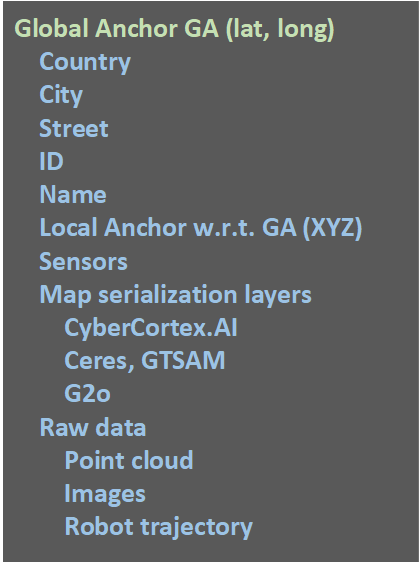
\includegraphics[scale=1.0]{map_indexing.png}
		\caption{\textbf{Map indexing} based on a Global Anchor. The map serialization layers are created based on the robot's sensors and SLAM algorithm.}
        \label{fig:map_indexing}
	\end{center}
\end{figure}

\subsection{Map Serialization}
\label{sec:map_serialization}


\section{Implementation}
\label{sec:implementation}

\begin{figure}
	\centering
	\begin{center}
		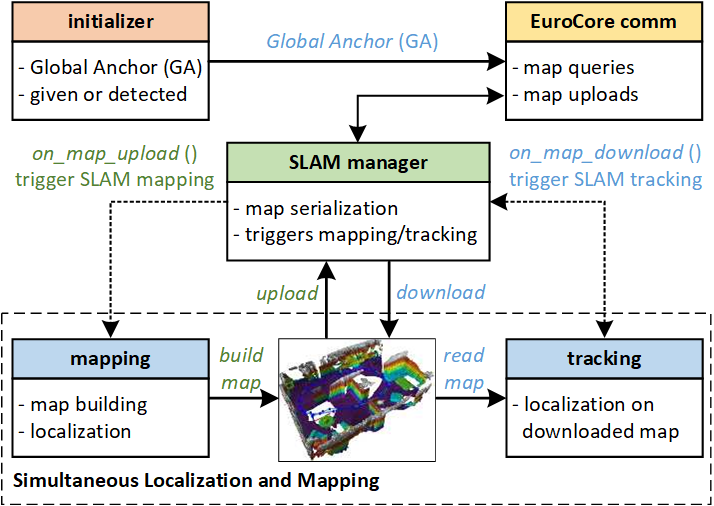
\includegraphics[scale=1.0]{overview.png}
		\caption{\textbf{NavGraph inference system onboard a robot}. The initializer is used to position the robot on the global map and trigger a map query from EuroCore. The SLAM manager de/serializes maps and triggers the SLAM algorithm.}
        \label{fig:overview}
	\end{center}
\end{figure}

\subsection{CyberCortex.AI Operating System}
\label{sec:cyc_os}

Autonomous robots and advanced automation systems rely on specialized Operating Systems (OS) that can schedule perception-and-control tasks and support real-time data exchange with other robots and remote cloud infrastructures. In our work, we use CyberCortex.AI, a robotics OS engineered for heterogeneous AI-driven robotics and complex automation. CyberCortex.AI is a decentralized, distributed operating system that allows robots to communicate seamlessly with each other as well as with high-performance computing (HPC) resources in the cloud.

Robot sensory and control data are continuously streamed to HPC platforms, where AI models are trained and then deployed back to the robots. Each robotic function—such as sensor data acquisition, path planning, or motion control—is encapsulated in a \textit{DataBlock of Filters}, which can be executed locally on the robot or remotely on another robotic system. Data exchange across filters is managed by a \textit{Temporal Addressable Memory} (TAM), which serves as the intermediary between inputs and outputs.

CyberCortex.AI is built around two core components: \textit{i}) the CyberCortex.AI inference system – a real-time DataBlock implementation running on embedded robotic hardware, and \textit{ii}) the CyberCortex.AI dojo – a cloud-based HPC environment for designing, training, and deploying AI algorithms.

\section{Conclusions}
\label{sec:conclusions}



%\nocite{*}
\bibliographystyle{IEEEtran}
\bibliography{references}


% that's all folks
\end{document}
